\documentclass{beamer}
%\usetheme(Goettingen}

\title{Chapitre 14 : Emission et Percéption d'un son}
\author{ROSALIE}
\date{\today}

\usepackage{tikz}
\usepackage{array}
\usepackage{siunitx}
 \sisetup{
    detect-all,
    output-decimal-marker={,},
    group-minimum-digits = 3,
    group-separator={~},
    number-unit-separator={~},
    inter-unit-product={~}
    }
\usepackage{pgf}

\begin{document}
	\maketitle
	
	\begin{frame}
	\frametitle{Introduction}
\begin{table}
	\begin{tabular}{c>{\centering}m{3cm}c}
		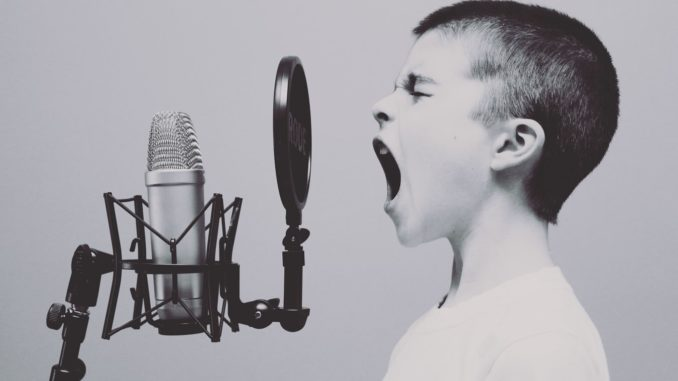
\includegraphics[scale=.15]{Ressources/Voix.jpg}&Quel est le point commun entre ces images ?&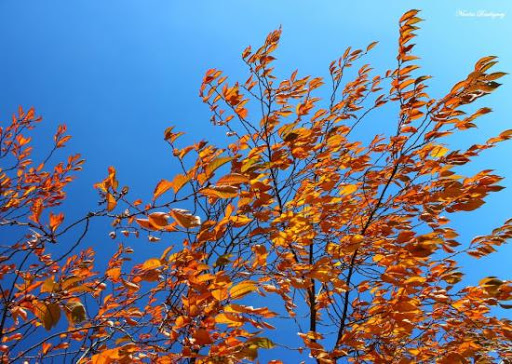
\includegraphics[scale=.165]{Ressources/unnamed.jpg}\\
		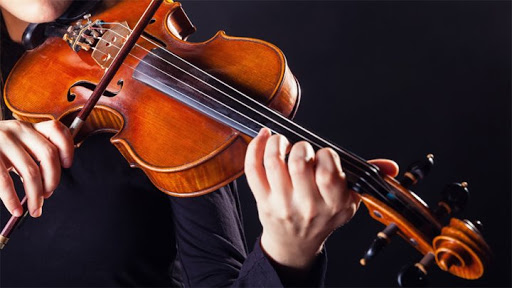
\includegraphics[scale=.2]{Ressources/violin.jpg}&\only<2>{\textbf{Le son}}&image d'eau qui coule\\
	\end{tabular}
\end{table}
\end{frame}

\begin{frame}
	\frametitle{1. Produire un signal sonore}
	\framesubtitle{A. Émission d'un son}
	Un son est créé par la vibration rapide d'un objet (cordes de guitare, ailes d'un insecte, peau frappée ...).\\
	Cette vibration est souvent d'amplitude de l'ordre du micromètre au millimètre entraînant la formation d'un son de faible intensité. Il est donc nécessaire d'amplifier cette vibration grâce à la caisse de résonance.
	\begin{figure}
	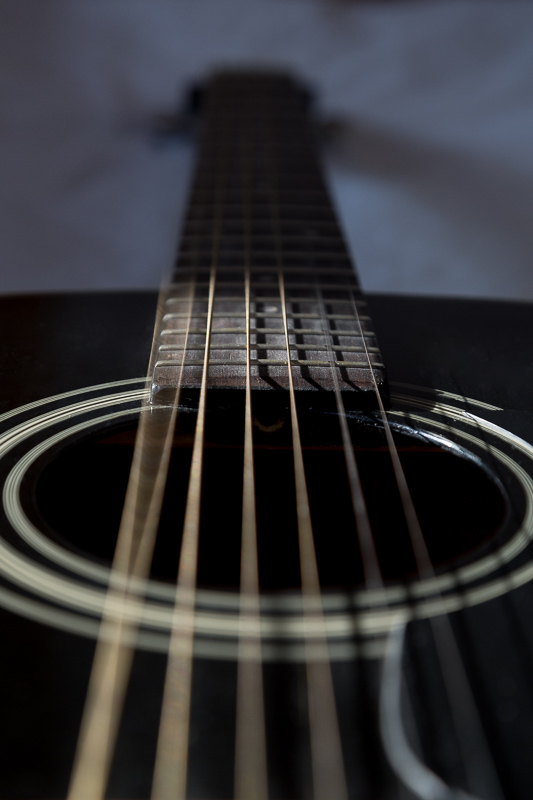
\includegraphics[scale=.12]{Ressources/Guitar.jpg} \hspace{2em}
	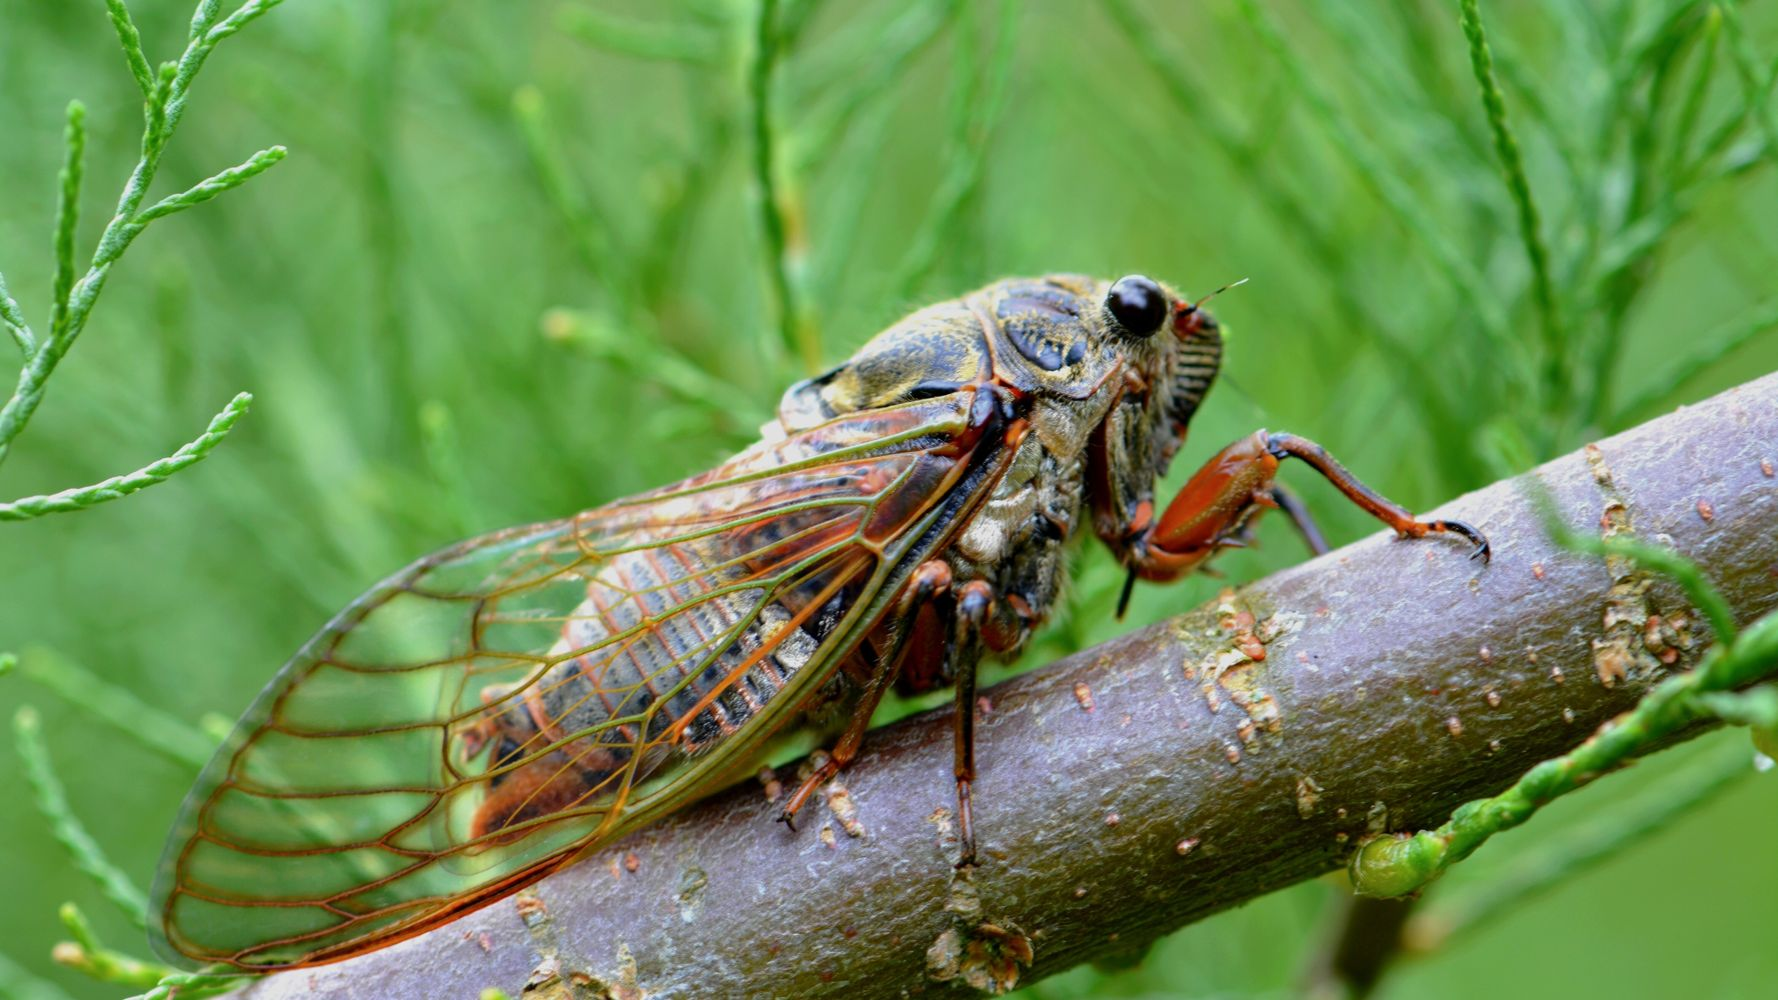
\includegraphics[scale=.07]{Ressources/Cigales.jpeg}
	\end{figure}
\end{frame}

\begin{frame}
	\frametitle{1. Produire un signal sonore}
	\framesubtitle{B. Propagation d'un son}
	Un son est perçu à distance de la source qui l'émet (distance séparant la source sonore de l'oreille). La vibration est donc transmise de proche en proche sans que la source n'ait à se déplacer. Un signal sonore est donc un phénomène de déplacement d'une perturbation de proche en proche dans un milieu matériel et sans transport effectif de matière.\\
	Il est donc nécessaire à une onde pour se propager de disposer d'un milieu matériel (exemple : air, bois, métal, eau ou tout autre matériau). En l'absence d'un milieu matériel, il ne peut pas y avoir propagation du son.
\end{frame}

\begin{frame}
	\frametitle{1. Produire un signal sonore}
	\framesubtitle{C. Vitesse de propagation du son : la célérité}
	La vitesse du son dans un milieu donné est caractéristique du milieu. Cette célérité dépend de la \textbf{nature du milieu} et de la \textbf{température}. Dans l'air, vers \SI{20}{\celsius}, la célérité du son est proche de \SI{340}{\meter\per\second}.
	\\
	
	\begin{tabular}{|>{\centering}m{2cm}|>{\centering}m{1cm}|>{\centering}m{2cm}|>{\centering}m{2cm}|>{\centering\arraybackslash}m{2cm}|}
		\hline \textbf{Milieu}& Air & Eau liquide & Verre & Acier\\
		\hline \textbf{$\mathbf{v}$ (\unit{\meter\per\second})} & \num{340} & \num{1500} &\num{5300}&\num{5800}\\
		\hline
	\end{tabular}
\end{frame}

\begin{frame}
	\frametitle{1. Produire un signal sonore}
	\framesubtitle{C. Vitesse de propagation du son : la célérité}
	\begin{small}
		\begin{tabular}{|>{\centering}m{2cm}|>{\centering}m{1cm}|>{\centering}m{2cm}|>{\centering}m{2cm}|>{\centering\arraybackslash}m{2cm}|}
			\hline \textbf{Milieu}& Air & Eau liquide & Verre & Acier\\
			\hline \textbf{$\mathbf{v}$ (\unit{\meter\per\second})} & \num{340} & \num{1500} &\num{5300}&\num{5800}\\
			\hline
		\end{tabular}
	\end{small}	
\vspace{1cm}

\underline{Exercice d'application :}\\
On place les deux enceintes d’une radio devant deux milieux différents, un aquarium
de 15m de long et un bloc de verre de même dimensions. Quel écart de temps va
séparer la perception du son à l’autre bout de l’aquarium et du bloc de verre ?
	
\end{frame}

\begin{frame}
	\frametitle{1. Produire un signal sonore}
	\framesubtitle{C. Vitesse de propagation du son : la célérité}
	Il faut comparer les temps pris par le son pour parcourir la distance de \SI{15}{m} dans chacun des matériaux.\\
	$v_{eau} = \dfrac{d}{\Delta t_{eau}}$ donc $\Delta t_{eau} = \dfrac{d}{v_{eau}} = \dfrac{15}{1500}$ = \SI{0,01}{s} = \SI{10}{ms}.\\
	
	$v_{verre} = \dfrac{d}{\Delta t_{verre}}$ donc $\Delta t_{verre} = \dfrac{d}{v_{verre}} = \dfrac{15}{5300}$ = \SI{0,003}{s} = \SI{3}{ms}.\\
	\vspace{1cm}
	Le son propagé dans le verre arrivera avant celui propagé dans l'eau. Le retard peut se calculer de la manière suivante :\\
	$retard=\Delta t_{eau} - \Delta t_{verre} = 10-3$ = \SI{7}{ms}.
\end{frame}

\begin{frame}
	\frametitle{2. Description d'un signal sonore}
	\framesubtitle{A. Représentation temporelle}
	\begin{minipage}{.4\linewidth}
	Avec un système d'acquisition, on peut visualiser la représentation temporelle d'un signal sonore.\\ \vspace{1em}
	Lorsque la représentation temporelle correspond à la représentation d'un motif élémentaire, on dit qu'elle est \textbf{périodique}.
	\end{minipage}
	\begin{minipage}{.55\linewidth}
		\centering
		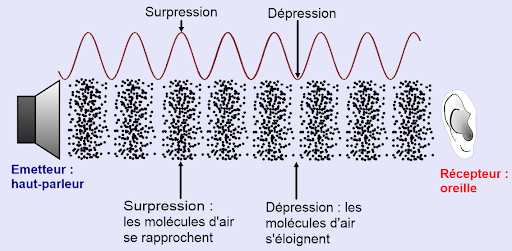
\includegraphics[width=\linewidth]{Ressources/haut parleur.png}\\ \vspace{1em}
		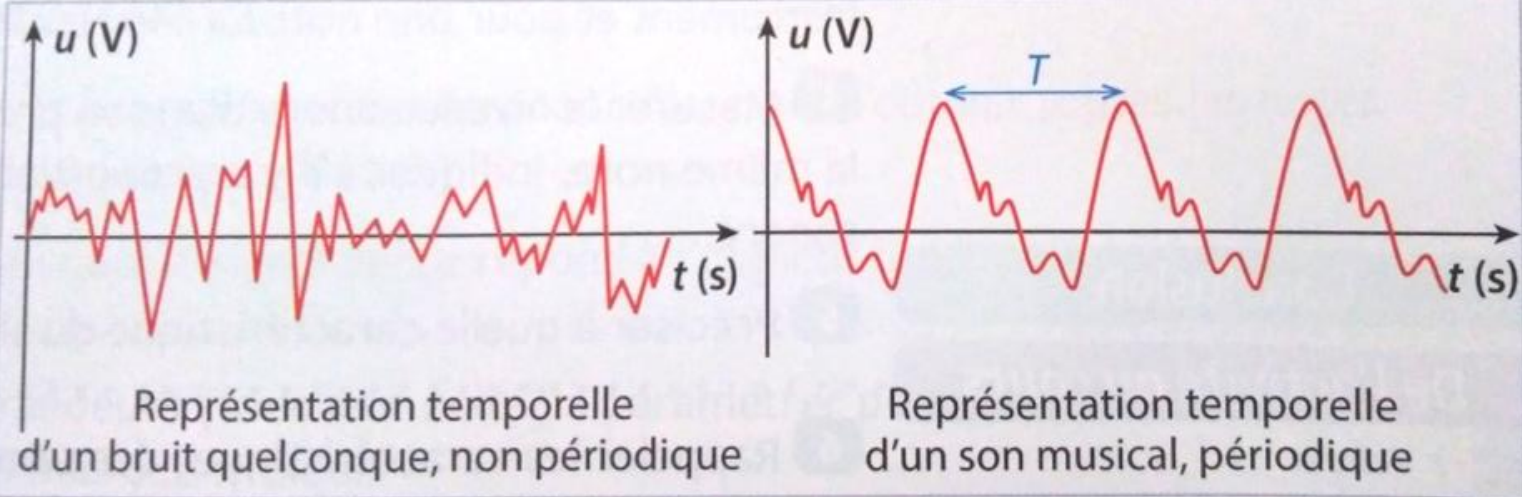
\includegraphics[width=\linewidth]{Ressources/2GT_C7_Fig1.png}
	\end{minipage}
\end{frame}

\begin{frame}
	\frametitle{2. Description d'un signal sonore}
	\framesubtitle{B. Période et fréquence d'un signal sonore}
	La \textbf{période $T$} d'un signal est la durée en seconde (s) d'un motif élémentaire.\\
	La \textbf{fréquence $\mathbf{f}$} du signal correspond au nombre de répétitions du motif élémentaire par seconde.
	$$f=\dfrac{1}{T}$$
	$f$, la fréquence en hertz (\unit{\hertz})\\
	$T$, la période en secondes (\unit{\second})
	
	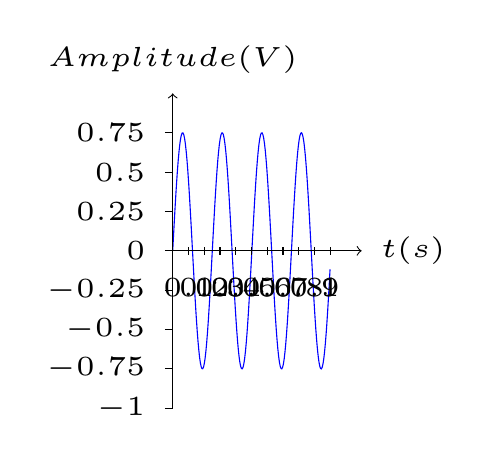
\begin{tikzpicture}[scale=2, transform shape]
		\draw [domain=0:1,samples = 200, color = blue] plot(\x,{.75*sin(25*\x r)});
		\draw[->] (0,0) -- (1.2,0);
		\draw (1.2,0) node[right] {\tiny $t (s)$};
		\draw[->] (0,-1) -- (0,1);
		\draw (0,1) node[above] {\tiny $Amplitude (V)$};
		\foreach \i in {-1,-0.75,...,.75}{
			%\pgfmathsetmacro\y{}
			\draw (-.05,\i)--(0,\i);
			\node[left] (n2) at (-.05,\i){\tiny \pgfmathprintnumber[precision=2]{\i}};
			%\draw (-.05,\i) node[left]{$A$};
		}
		\foreach \i in {.1,.2,...,1}{
			\draw (\i,-.025)--(\i,.025);
			\node[below] (n2) at (\i,-.05){\tiny \pgfmathprintnumber[precision=3]{\i}};
		}
		%\foreach \d in {0,1,...,6} {
        %\pgfmathsetmacro\y{13.3+0.05*\d}
        %\pgfkeys{/pgf/number format/.cd,fixed,fixed zerofill,precision=2}
        %\draw (-.1,\d)--(.1,\d);
        %\draw (0,\d) node[left]{\pgfmathprintnumber[precision=2]{\y}};
        %\draw[gray] (-.1,\d)--(8,\d);
        %}
	\end{tikzpicture}

\end{frame}

\begin{frame}
	\frametitle{3. La perception d'un son}
	\framesubtitle{A. Domaine de fréquences}
	L'oreille humaine permet de dissocier les sons en fonction de leur fréquence.\\
	Elle ne peut entendre que les signaux sonores dont les fréquences sont comprises entre \SI{20}{\hertz} et \SI{20}{\kilo\hertz}.
	\begin{figure}[h!]
		\centering
		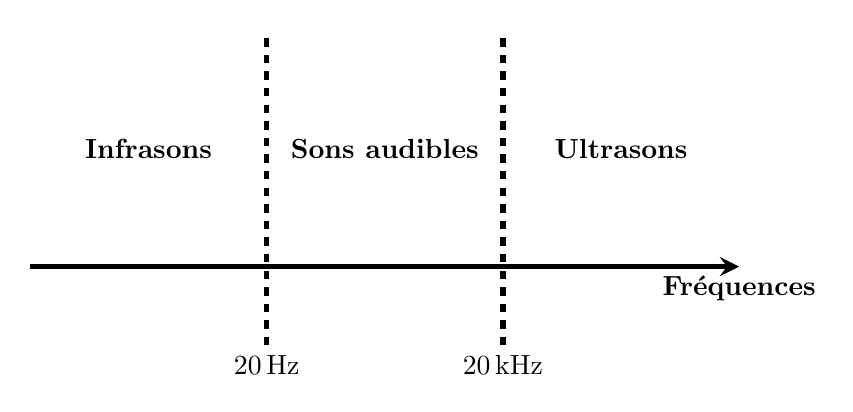
\begin{tikzpicture}
		\draw[line width =2pt,-stealth] (0,0) to (9,0); 
		\draw[dashed, line width = 2pt] (3,-1)--(3,3);
		\draw[dashed, line width = 2pt] (6,-1)--(6,3);
		\node[below] at (3,-1) {\SI{20}{Hz}};
		\node[below] at (6,-1) {\SI{20}{kHz}};
		\node at (1.5,1.5) {\textbf{Infrasons}};
		\node at (4.5,1.5) {\textbf{Sons audibles}};
		\node at (7.5,1.5) {\textbf{Ultrasons}};
		\node[below] at (9,0) {\textbf{Fréquences}};
		\end{tikzpicture}
	\end{figure}
\end{frame}

\begin{frame}
	\frametitle{3. La perception d'un son}
	\framesubtitle{B. Hauteur et timbre d'un son}
	Les sons émis par deux cordes différentes d'un violon ou deux touches d'un piano n'ont pas la même fréquence. Ils n'ont pas la même \textbf{hauteur}.\\
	La \textbf{hauteur} d'un son est la perception auditive procurée par son audition : plus la hauteur d'un son est aigüe, plus sa fréquence est élevée. 
\end{frame}

\begin{frame}
	\frametitle{3. La perception d'un son}
	\framesubtitle{B. Hauteur et timbre d'un son}
	Le timbre d'un son est quant à lui lié à la forme d'un signal sonore. 
\end{frame}
\begin{frame}
	\frametitle{3. La perception d'un son}
	\framesubtitle{C. Intensité et niveau d'intensité sonore}
	Plus l’amplitude d’un signal sonore est élevée, plus l’intensité sonore $I$ est grande. L’intensité sonore
	s’exprime en watt par mètre carré (\unit{\watt\per\meter\squared})
	Pour lier la sensibilité de l’oreille humaine à l’intensité d’un
	son, le niveau d’intensité sonore ($L$) exprimée en (\unit{\deci\bel} ) a été mise en place. Il s’agit de changer d’échelle.\\
	Le niveau d’intensité sonore se mesure à l’aide d’un
	sonomètre.
\end{frame}

\begin{frame}
	\frametitle{3. La perception d'un son}
	\framesubtitle{D. Exposition sonore}
	Les risques liés à l’exposition sonore sont	directement liés au niveau sonore et à la durée d’exposition.\\
	Une exposition sonore trop élevée
	peut avoir des conséquences
	irréversibles, comme une surdité partielle, voir totale.
\end{frame}
\end{document}